\graphicspath{{./Figs/}}

\chapter{Theory and Methodology}
This chapter outlines the theory and Methodology used create, test and collect the data required for the wing-propeller interaction analysis. 

\section{Material Choice}
In order to readily edit and modify the model to be tested 3D printing was used to print the final developed model. 3D printing has become increasingly common when developing models to be tested in wind tunnels. Polyatic acid (PLA) filament was used to print the main body of the model as this is the most widely used and avaliable filament for 3D printing purposes. It has a reasonably low melting point of $\approx$ 150 $^{\circ}$, good layer adhesion and it can also be extruded in a variety of ways in order to develop different textures on the surface of the 3D model. This is partiularly significant for MAVs as the surface of aircraft are typically smooth in order to reduce viscous drag effects. 3D printed models often have ridges between layers which have been printed. However \todo{Finish}


\section{FreeCAD}
FreeCAD is a 3D parametric modeler and was used with provided python scripts to produce fuselage, wing and tail shapes when given input parameters to define the shape and geometry. Various model shapes were produced with the aim of making the model 3D printable in order to allow for ease of manufacturing and testing. Several design constraints had to be considered when developing the model due to the structural strength of the PLA used for 3D-printing and the limitations. The wings and tail in particular could not be too thin or short in order to allow for the parts to be 3D printed while maintaining structural integrity. The main fuselage
\todo{finish + add photo}

The model was also fitted to mount into the 3x4 wind tunnel for testing as shown in Figure \todo{add figure here}

\section{VAP 3.5}
VAP 3.5 is a open-source software which uses the High-Order Free Wake (HOFW) \todo{abb} method in order to determine the aerodynamic performace of MAV designs. \\

The HOFW method


\section{XFOIL}
XFOIL is another open source free to use software which has been developed by Harold Youngren and Mark Drela. The software is used to analyse 2D airfoils for their aerodynamic characteristics. XFOIL was used to produce aerofoil data which accounted for viscous effects. It is essential that the software account for the viscous effects as this has an essential role in the flow characteristics accross the surface of an aircraft wing. This is especially true at low Reynolds numbers where the  \todo{finsiht this}. XFOIL accounts for the viscous effects by using the wake momentum thickness to determine the skin friction produced as fluid passes over the surface of the airfoil as given by Equation \ref{eqn:XFOIL}. 


\begin{equation}
    \theta = \int_{0}^{\infty} \frac{u}{U_e} ( 1 - \frac{u}{U_e) } \,dy
    \label{eqn:XFOIL}
\end{equation}

Where:
\begin{itemize}
    \item $\theta$ is the momentum thickness at a given point along the airfoil
    \item $U_e$ is the freestream velocity 
    \item u is the flow velocity at a position y distance from the airfoil surface
\end{itemize}

In this manner the skin friction losses can be determined and accounted for when running the VAP software to analyse the stability of the model. 

\section{Model Development}

\section{Wind Tunnel Testing}
In order to analyse the stability of the final developed model in the three configurations, the model was mounted in the wind tunnel to determine the forces and moments acting at several conditions in order to assess the effect that adding a propeller has on the stability of the model


\subsection{Wind Tunnel Setup}

Wind tunnel tests were taken for several variations of Aoa, airspeed, propeller speed and configuration. These are outlined below

\begin{itemize}
    \item Aoa: -5 $^{\circ}$ to 15 $^{\circ}$ in increments of 2$^{^circ}$
    \item Airspeed: 10m/s, 15m/s and 20m/s
    \item Motor speed: 6000RPM, 9000RPM, 11000RPM
    \item Configuration: No propeller, tractor and pusher
\end{itemize}

A safety net was placed in the wind tunnel in case any parts of the model were unable to remain attached as the airspeed increased to 20m/s.

\begin{figure}[!ht]
    \centering
    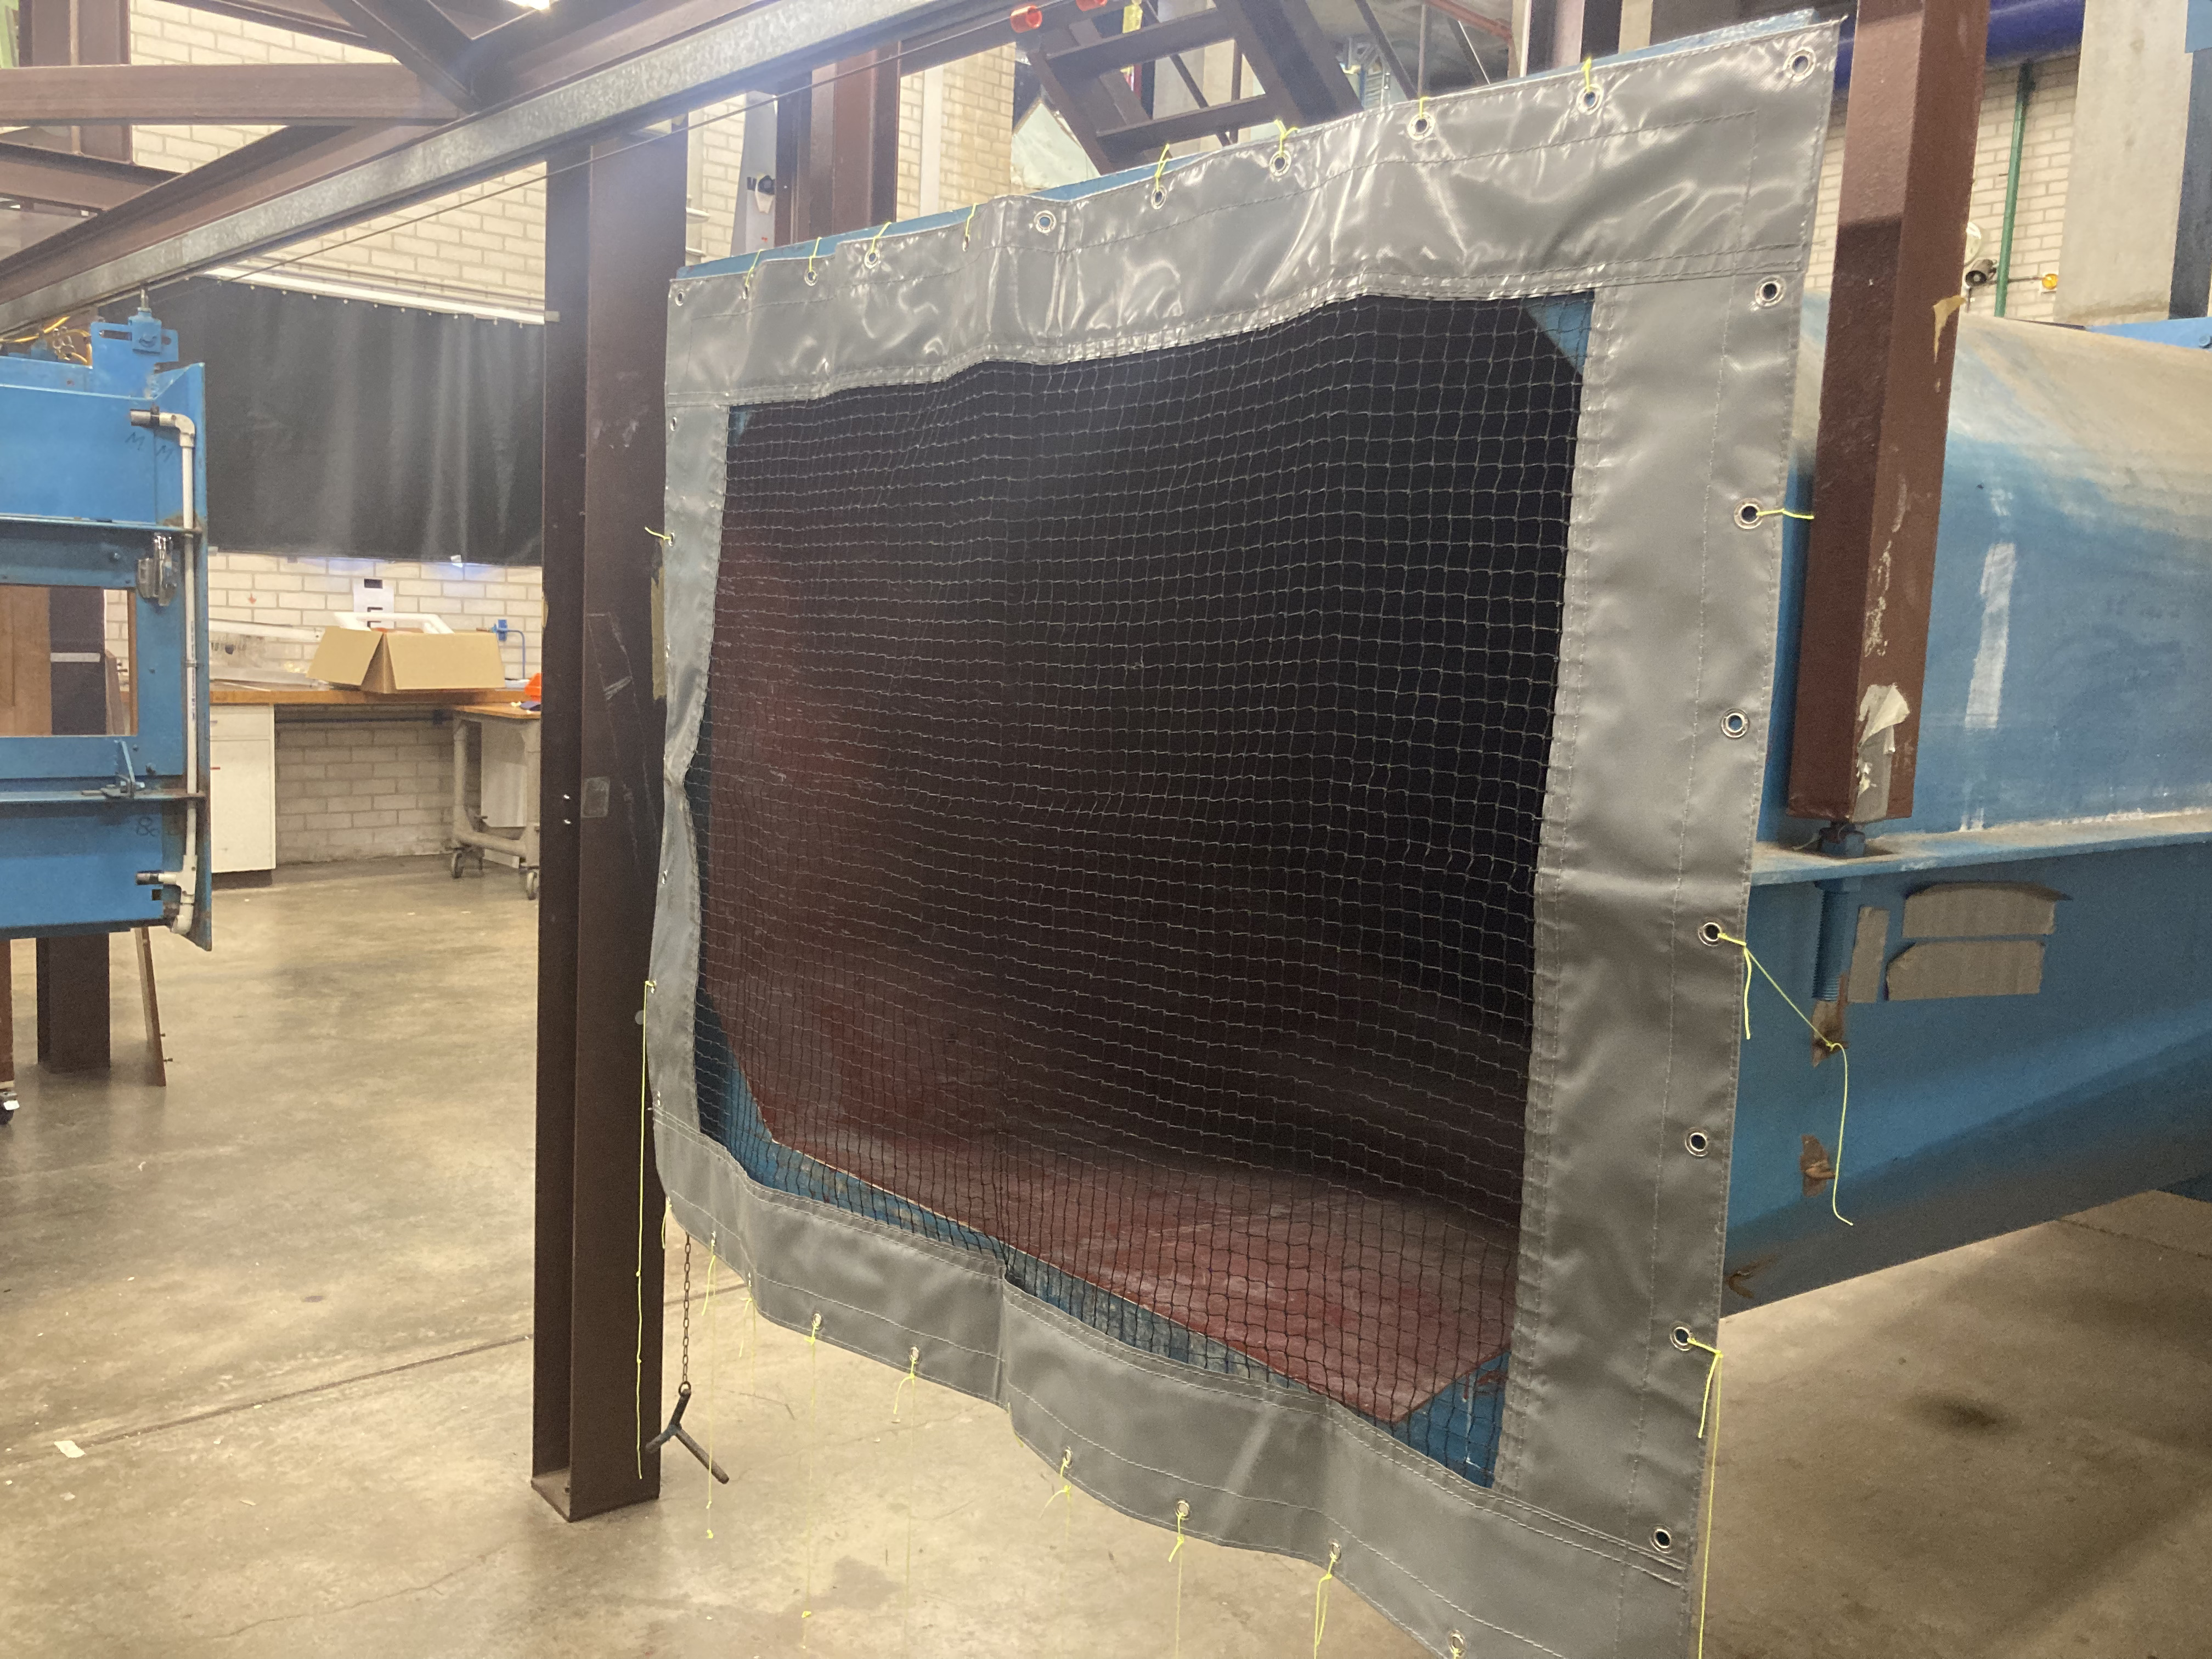
\includegraphics[scale =0.1]{04_Methodology/Figs/windTunnelNet.jpg}
    \caption{Safety net to }
    \label{fig:windTunnelNet}
\end{figure}

\begin{figure}[!ht]
    \centering
    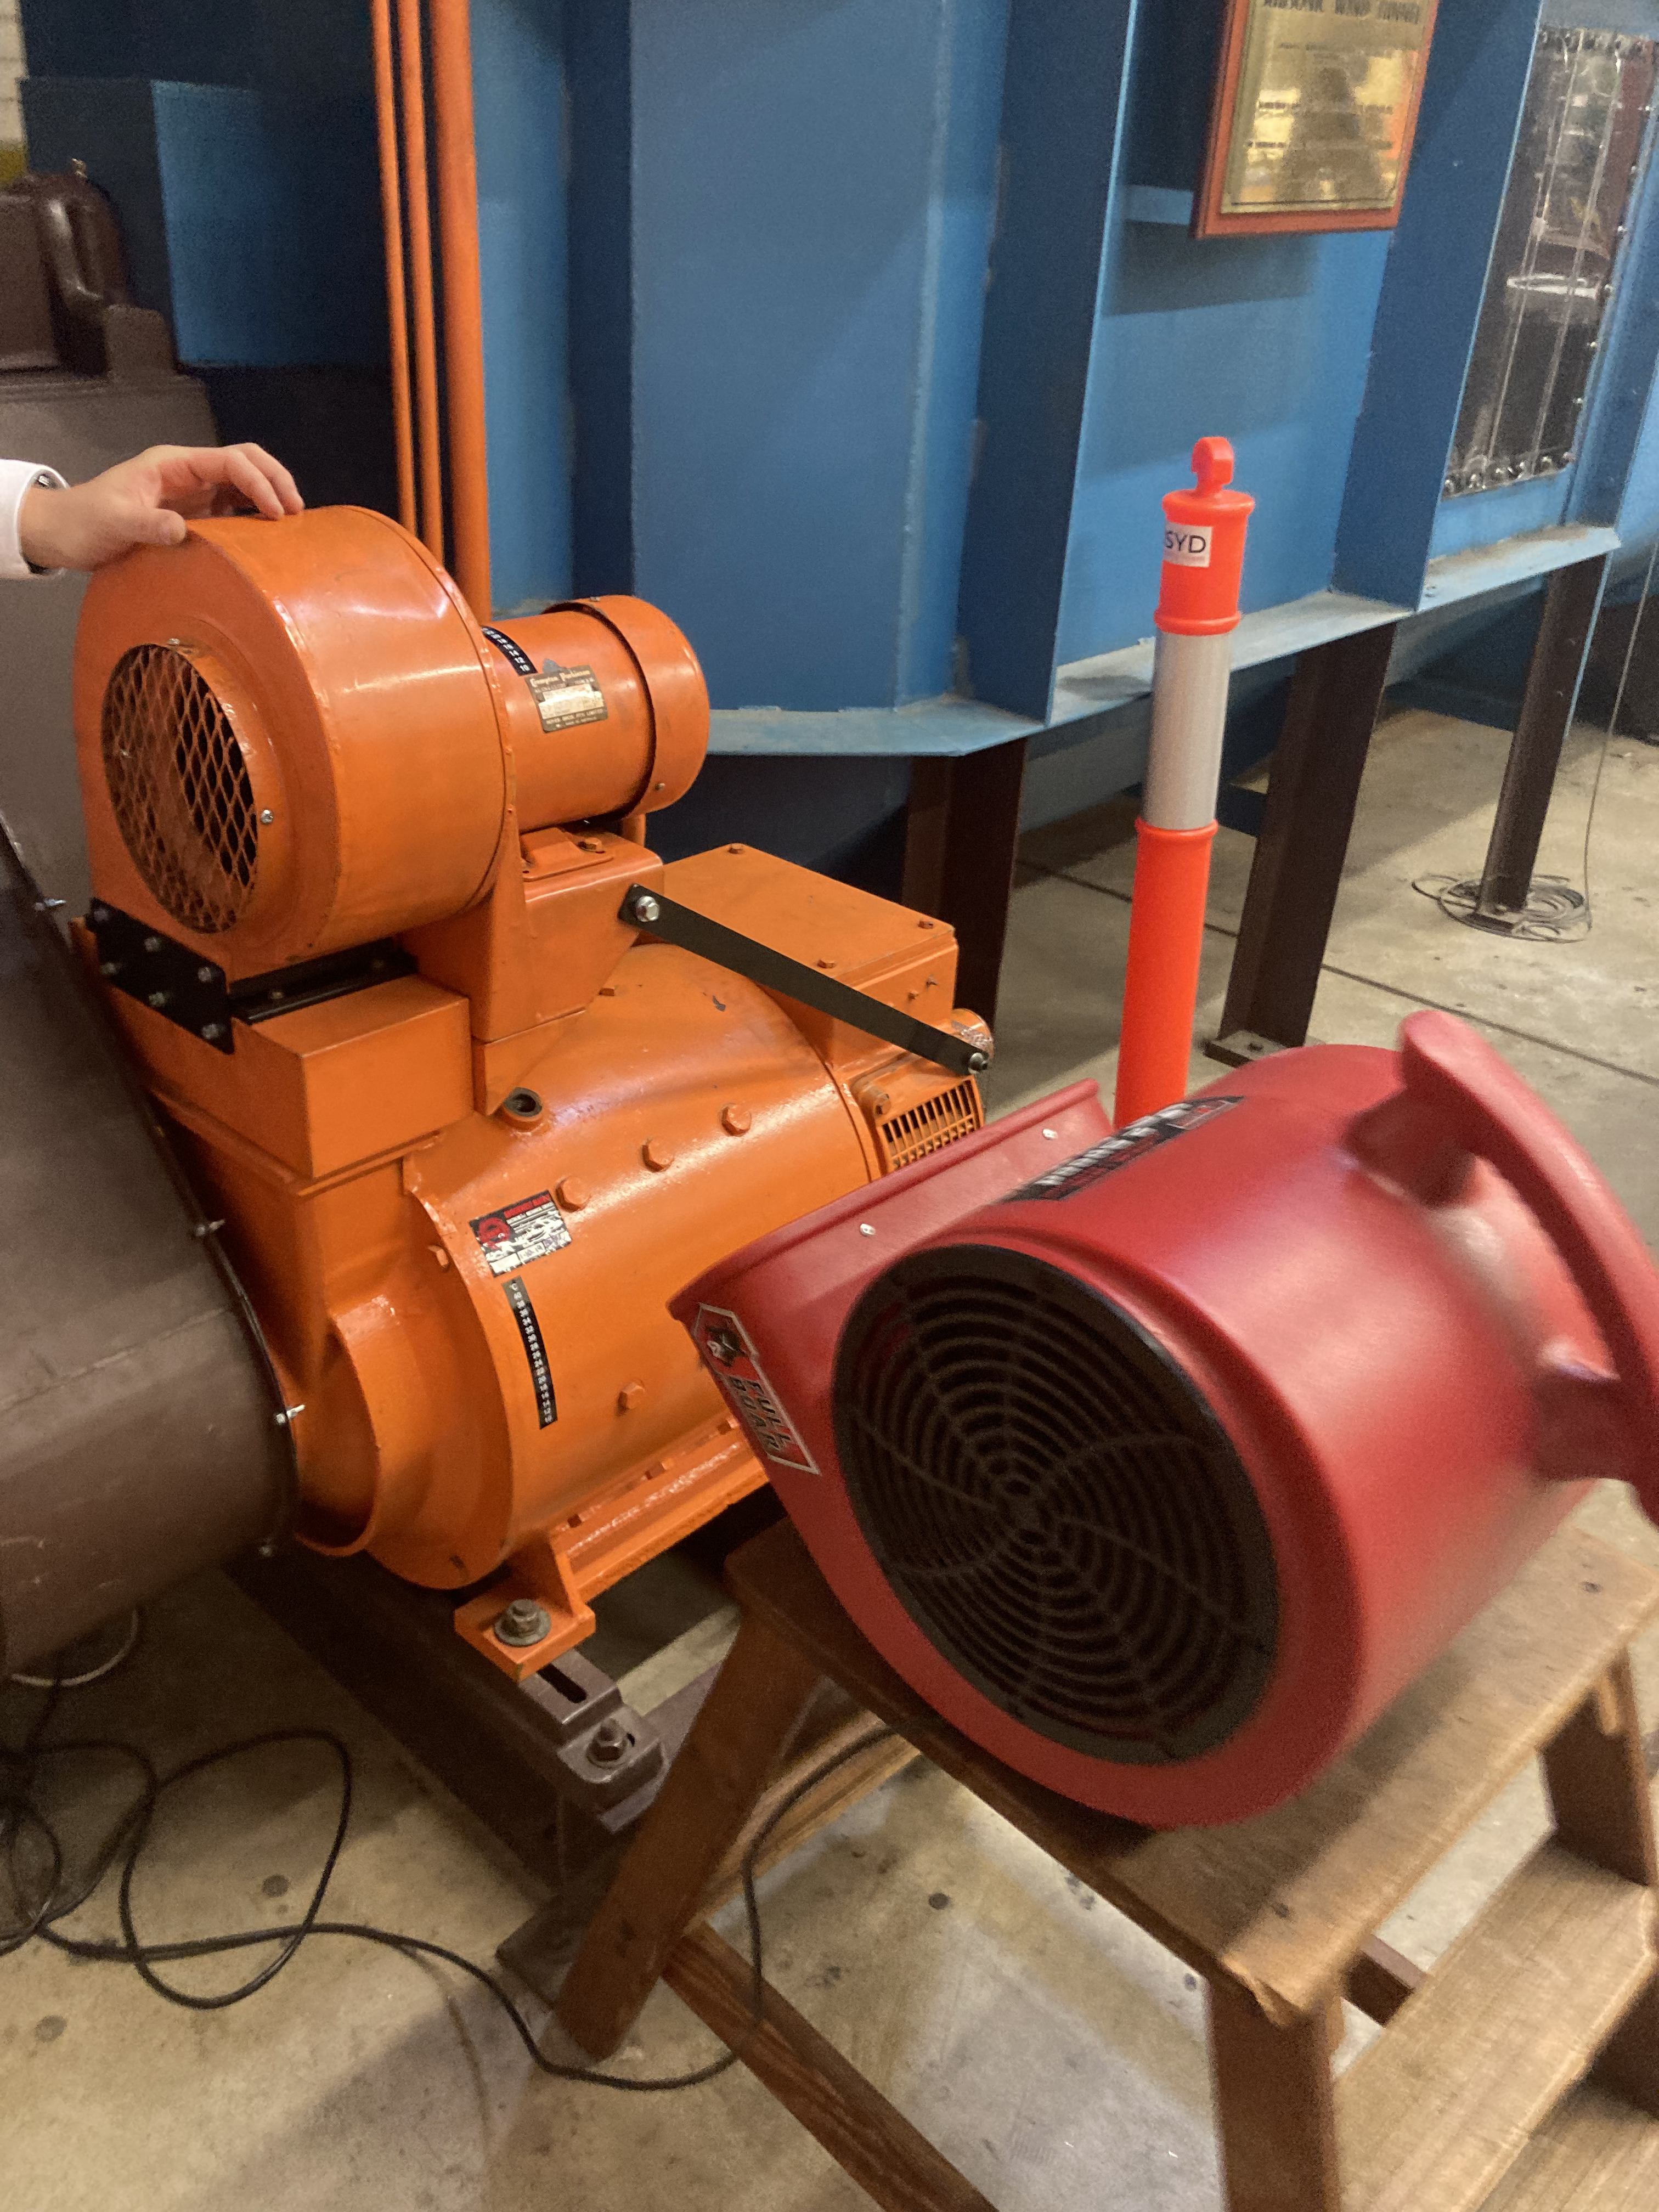
\includegraphics[scale=0.1]{04_Methodology/Figs/cooler.jpg}
    \caption{Caption}
    \label{fig:engineCooler}
\end{figure}

The nano25 load cell was used to record the forces and moments acting on the model about the mounting position at 25$\overline{c}$. 

\begin{figure}[H]
    \centering
    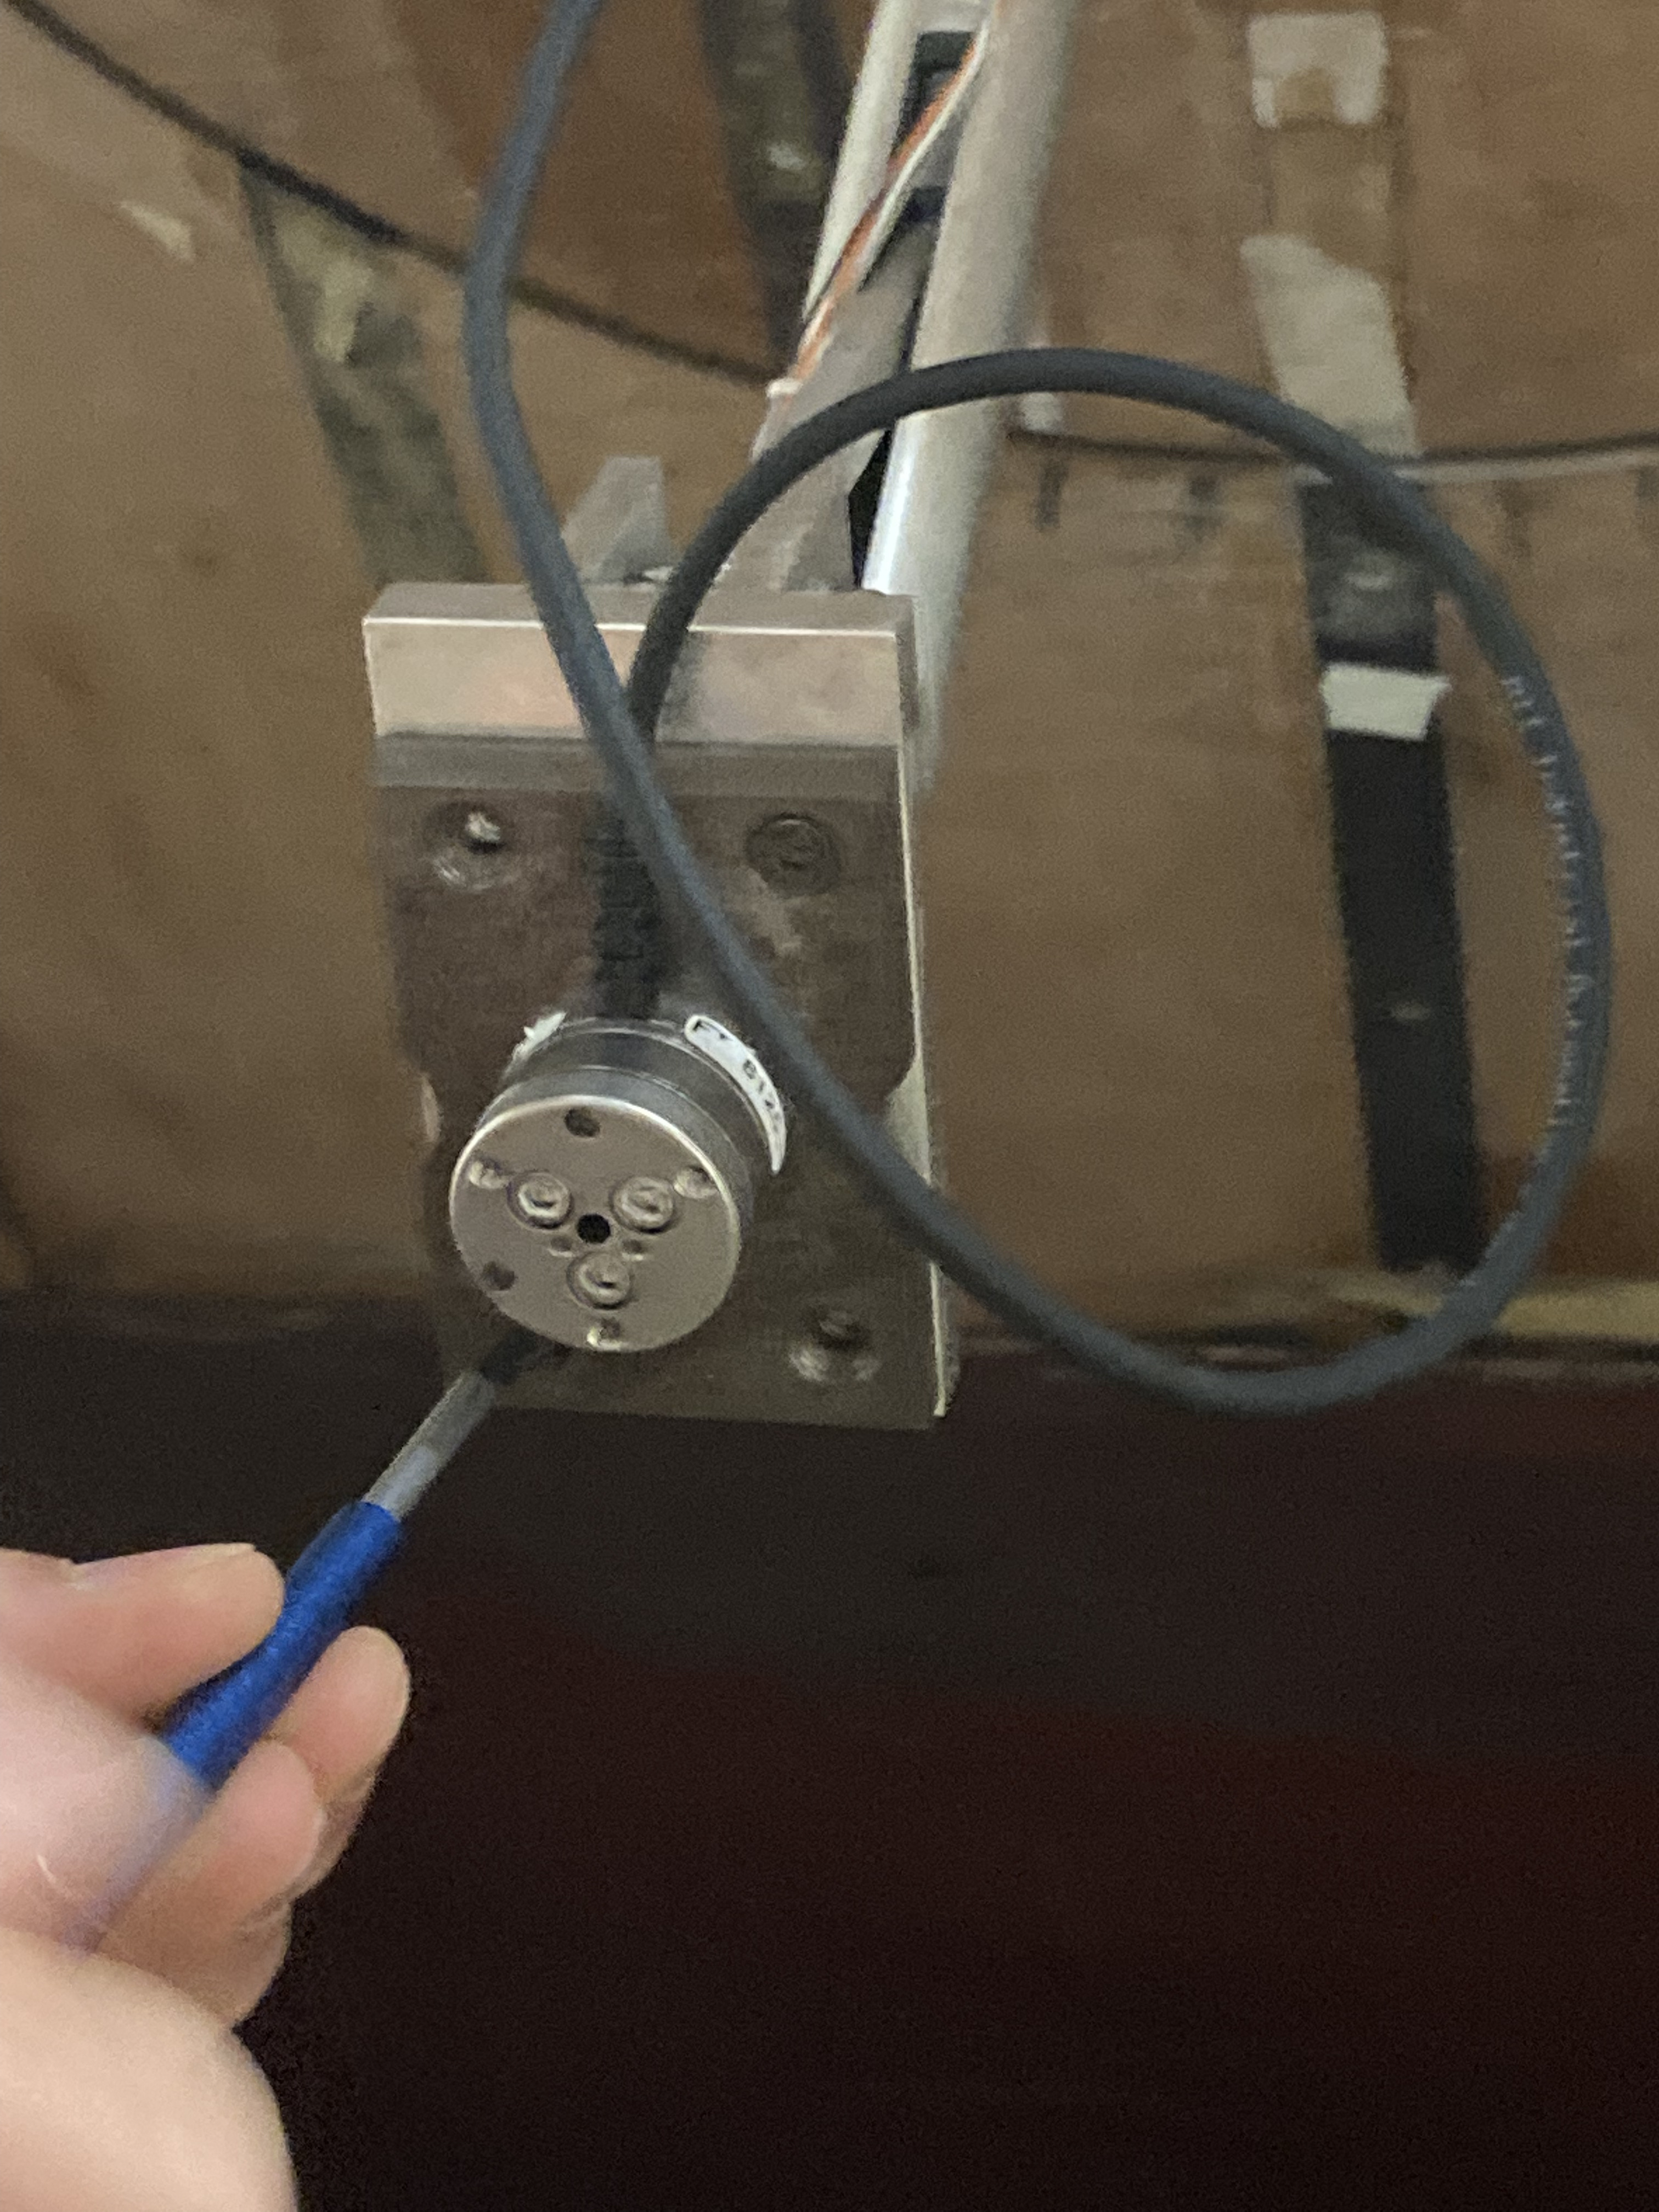
\includegraphics[scale=0.08]{04_Methodology/Figs/loadCellMount}
    \caption{Nano 25 load cell mount}
    \label{fig:LoadCella}
\end{figure}

The model mount was then attached over the load cell. 


\begin{figure}[!ht]
    \centering
    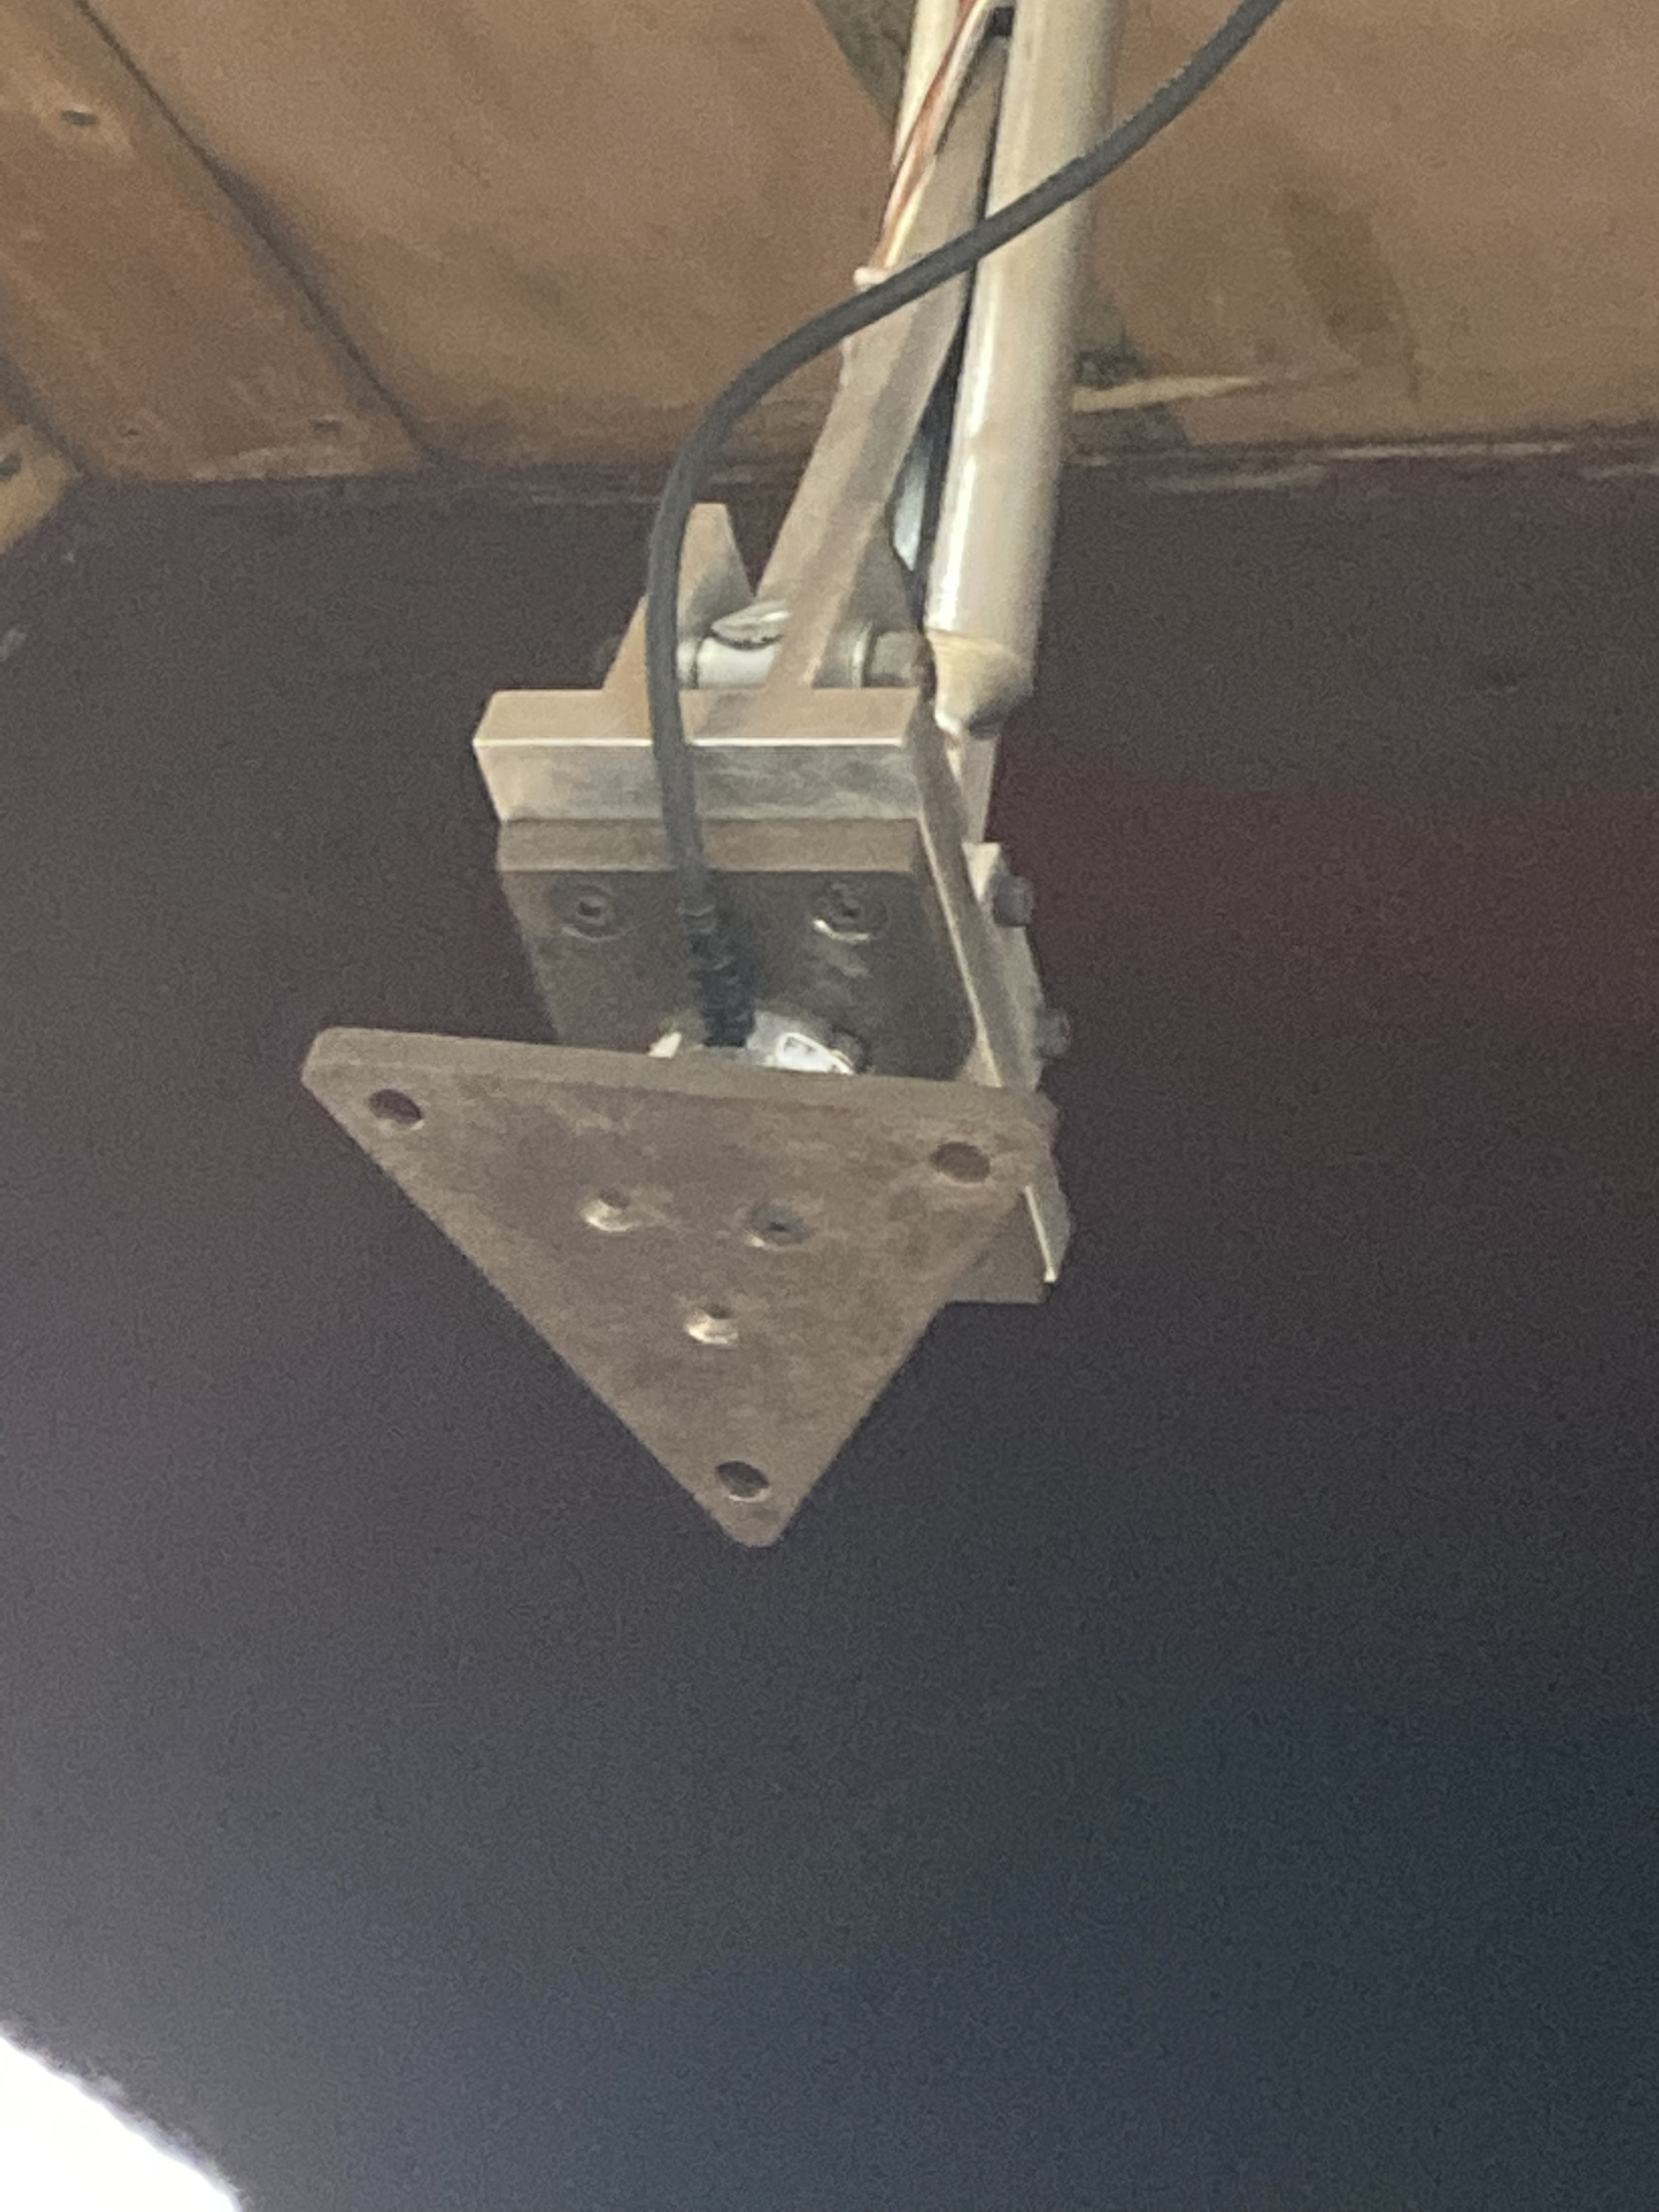
\includegraphics[scale=0.1]{04_Methodology/Figs/mount}
    \label{fig:LoadCellb}
\end{figure}

The model was then attached in three main configurations. These were mounting the propeller without a propeller, in a tractor and pusher configurations.


\begin{figure}[!ht]
     \centering
     \begin{subfigure}[b]{0.3\textwidth}
         \centering
         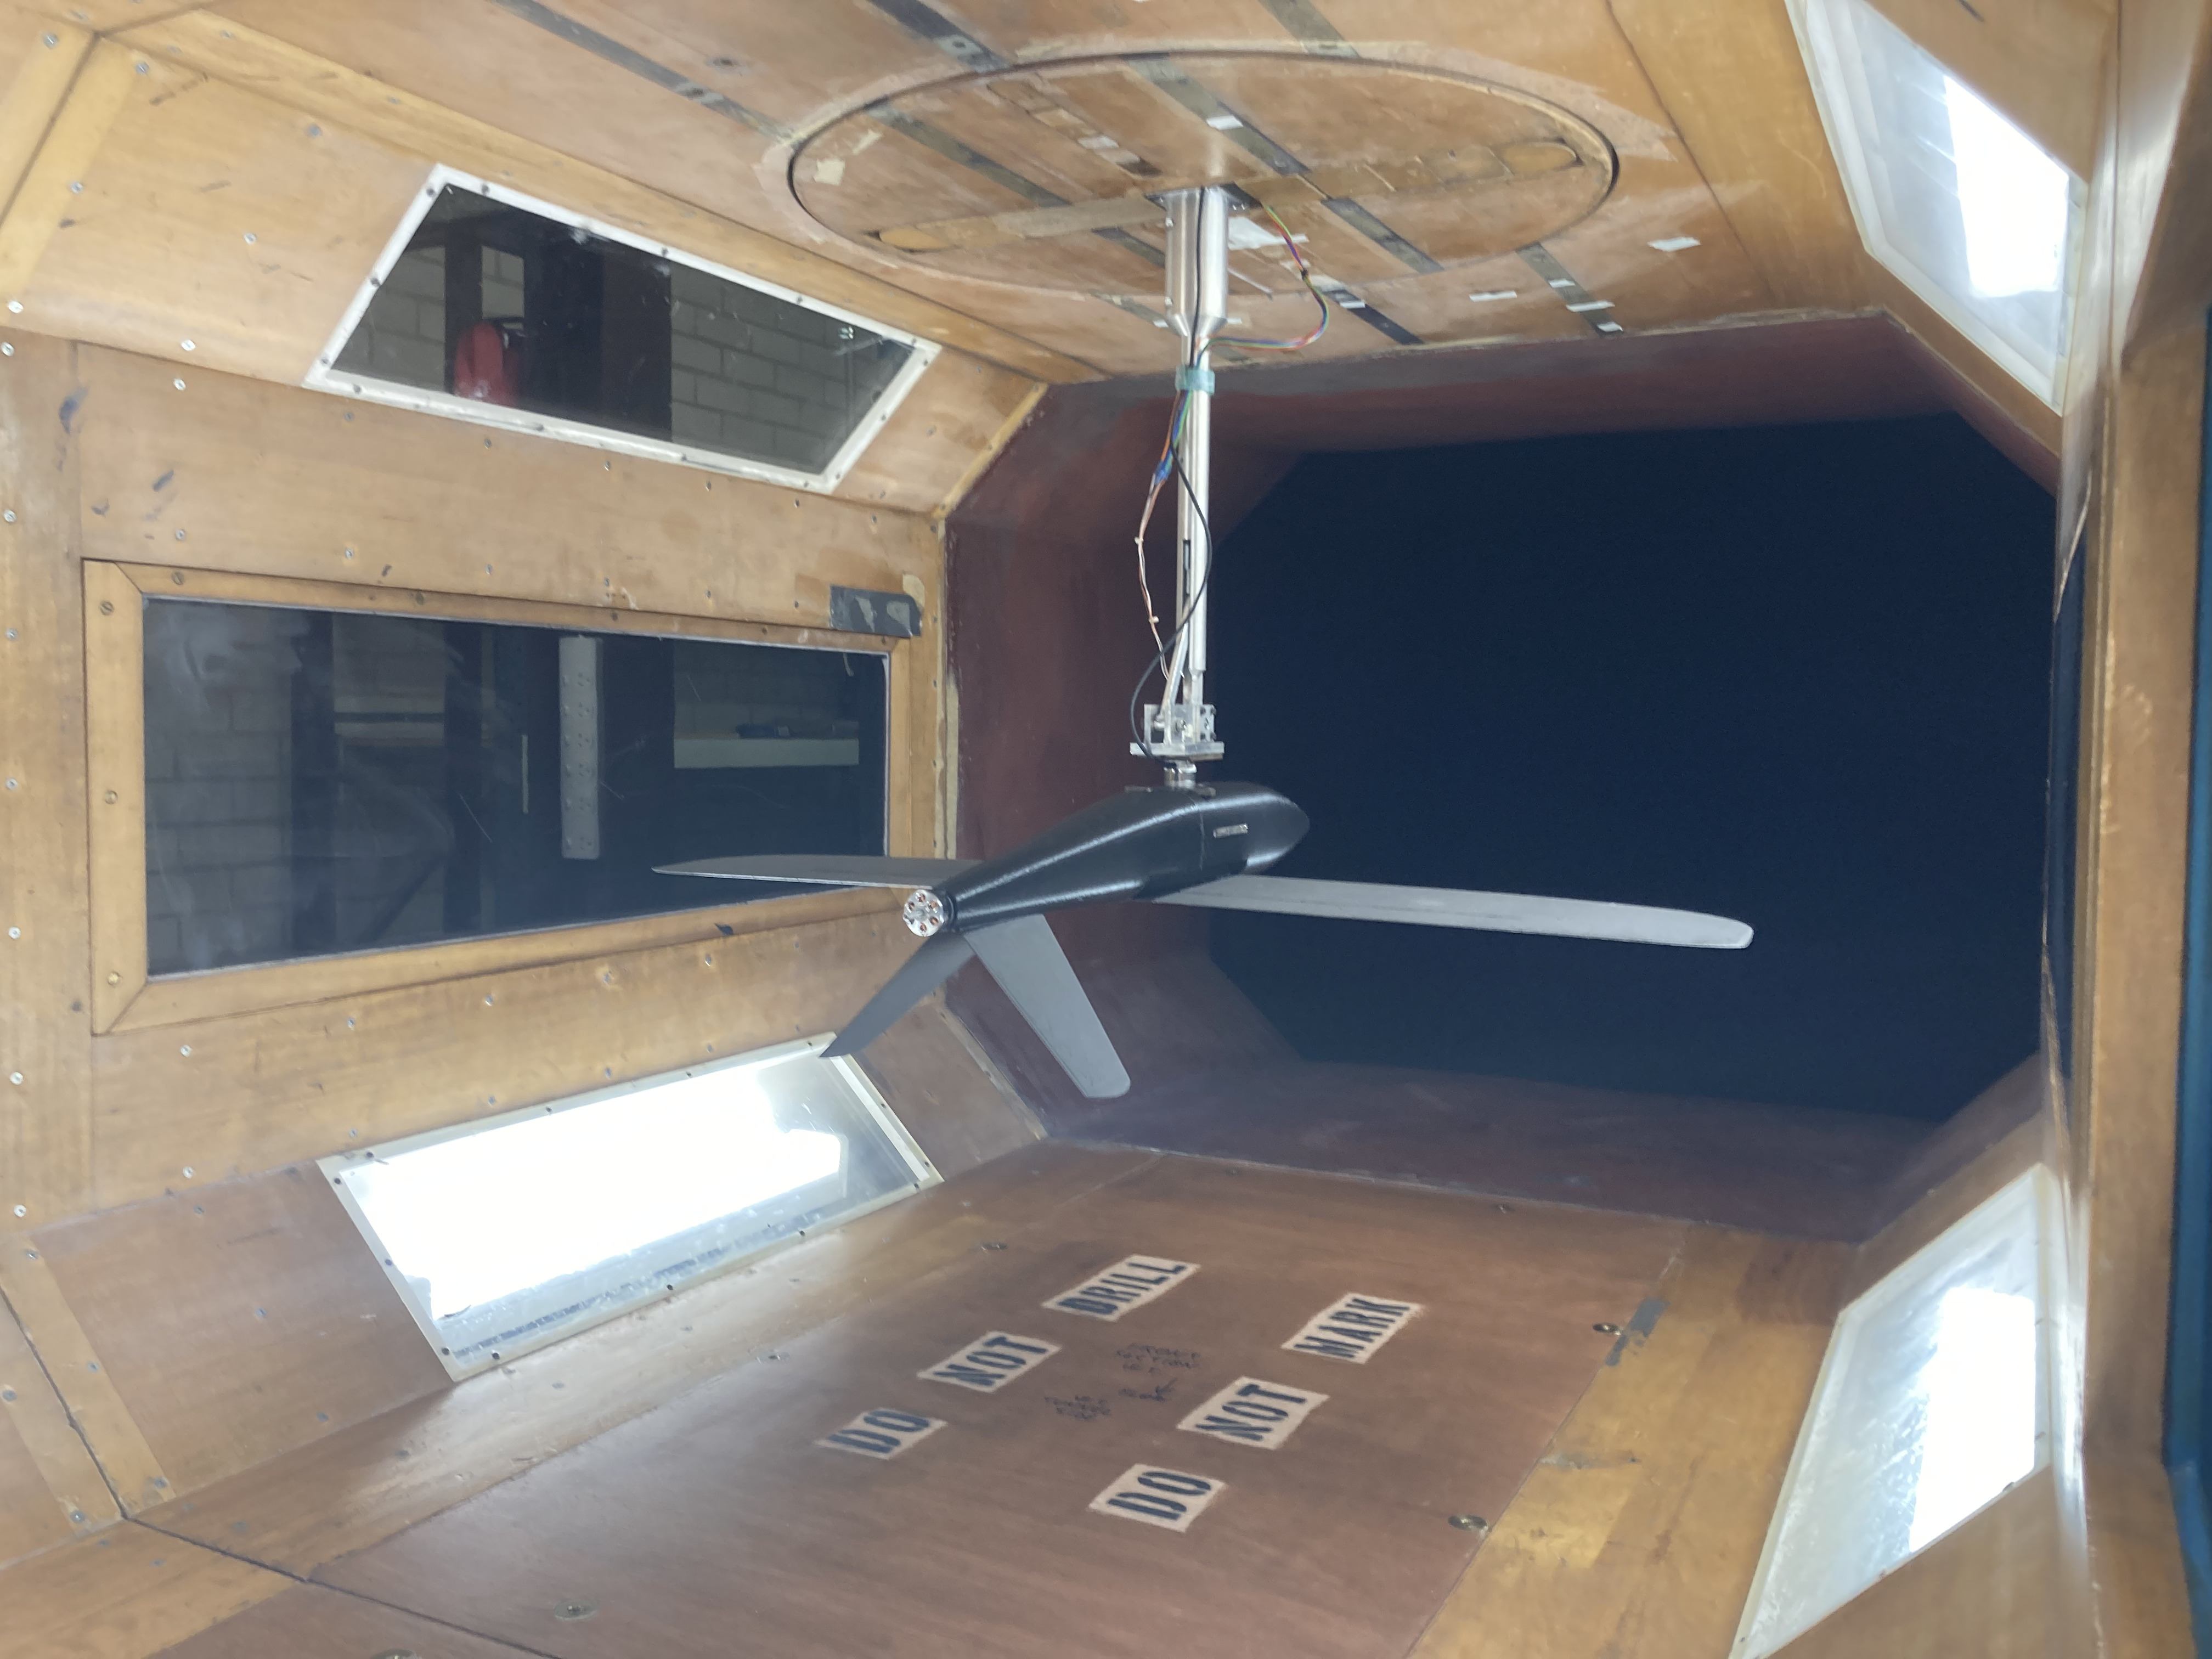
\includegraphics[scale=0.1]{04_Methodology/Figs/noprop}
          \label{fig:noprop}
     \end{subfigure}
     \hfill
     \begin{subfigure}[b]{0.3\textwidth}
             \centering
             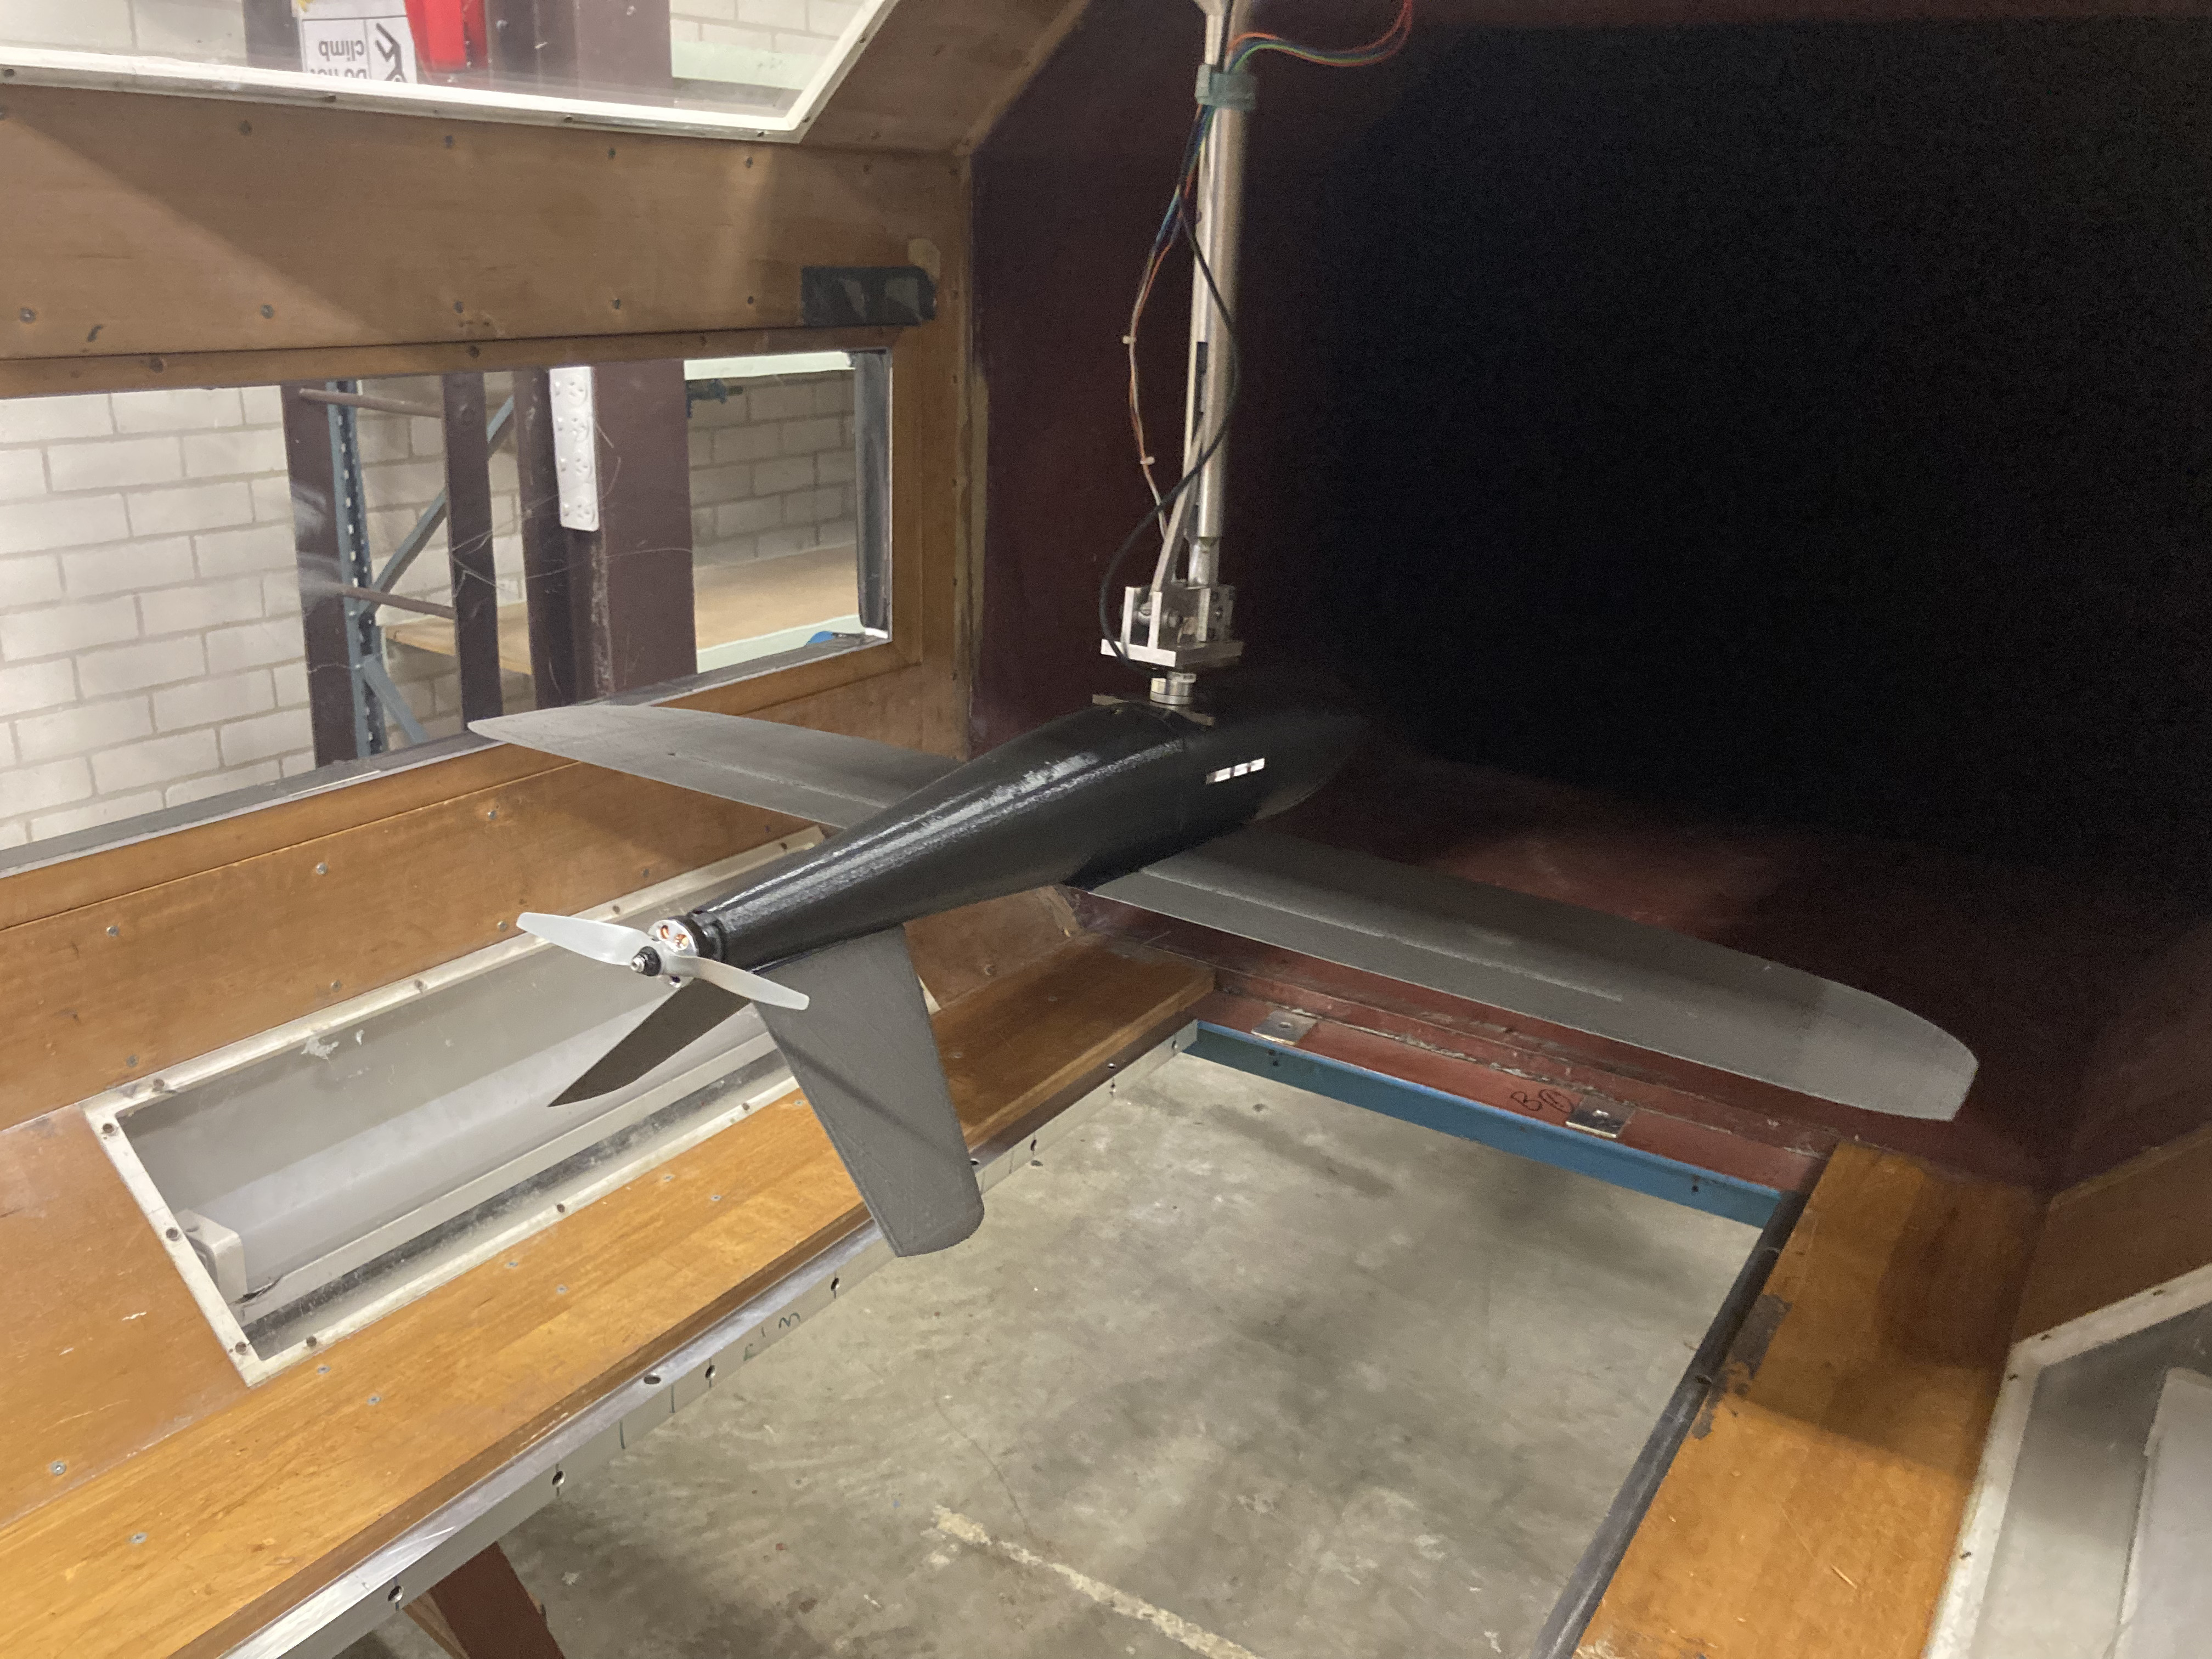
\includegraphics[scale = 0.1]{04_Methodology/Figs/pusher}
             \label{fig:pusher}
     \end{subfigure}
     \hfill
     \begin{subfigure}[b]{0.3\textwidth}
             \centering
             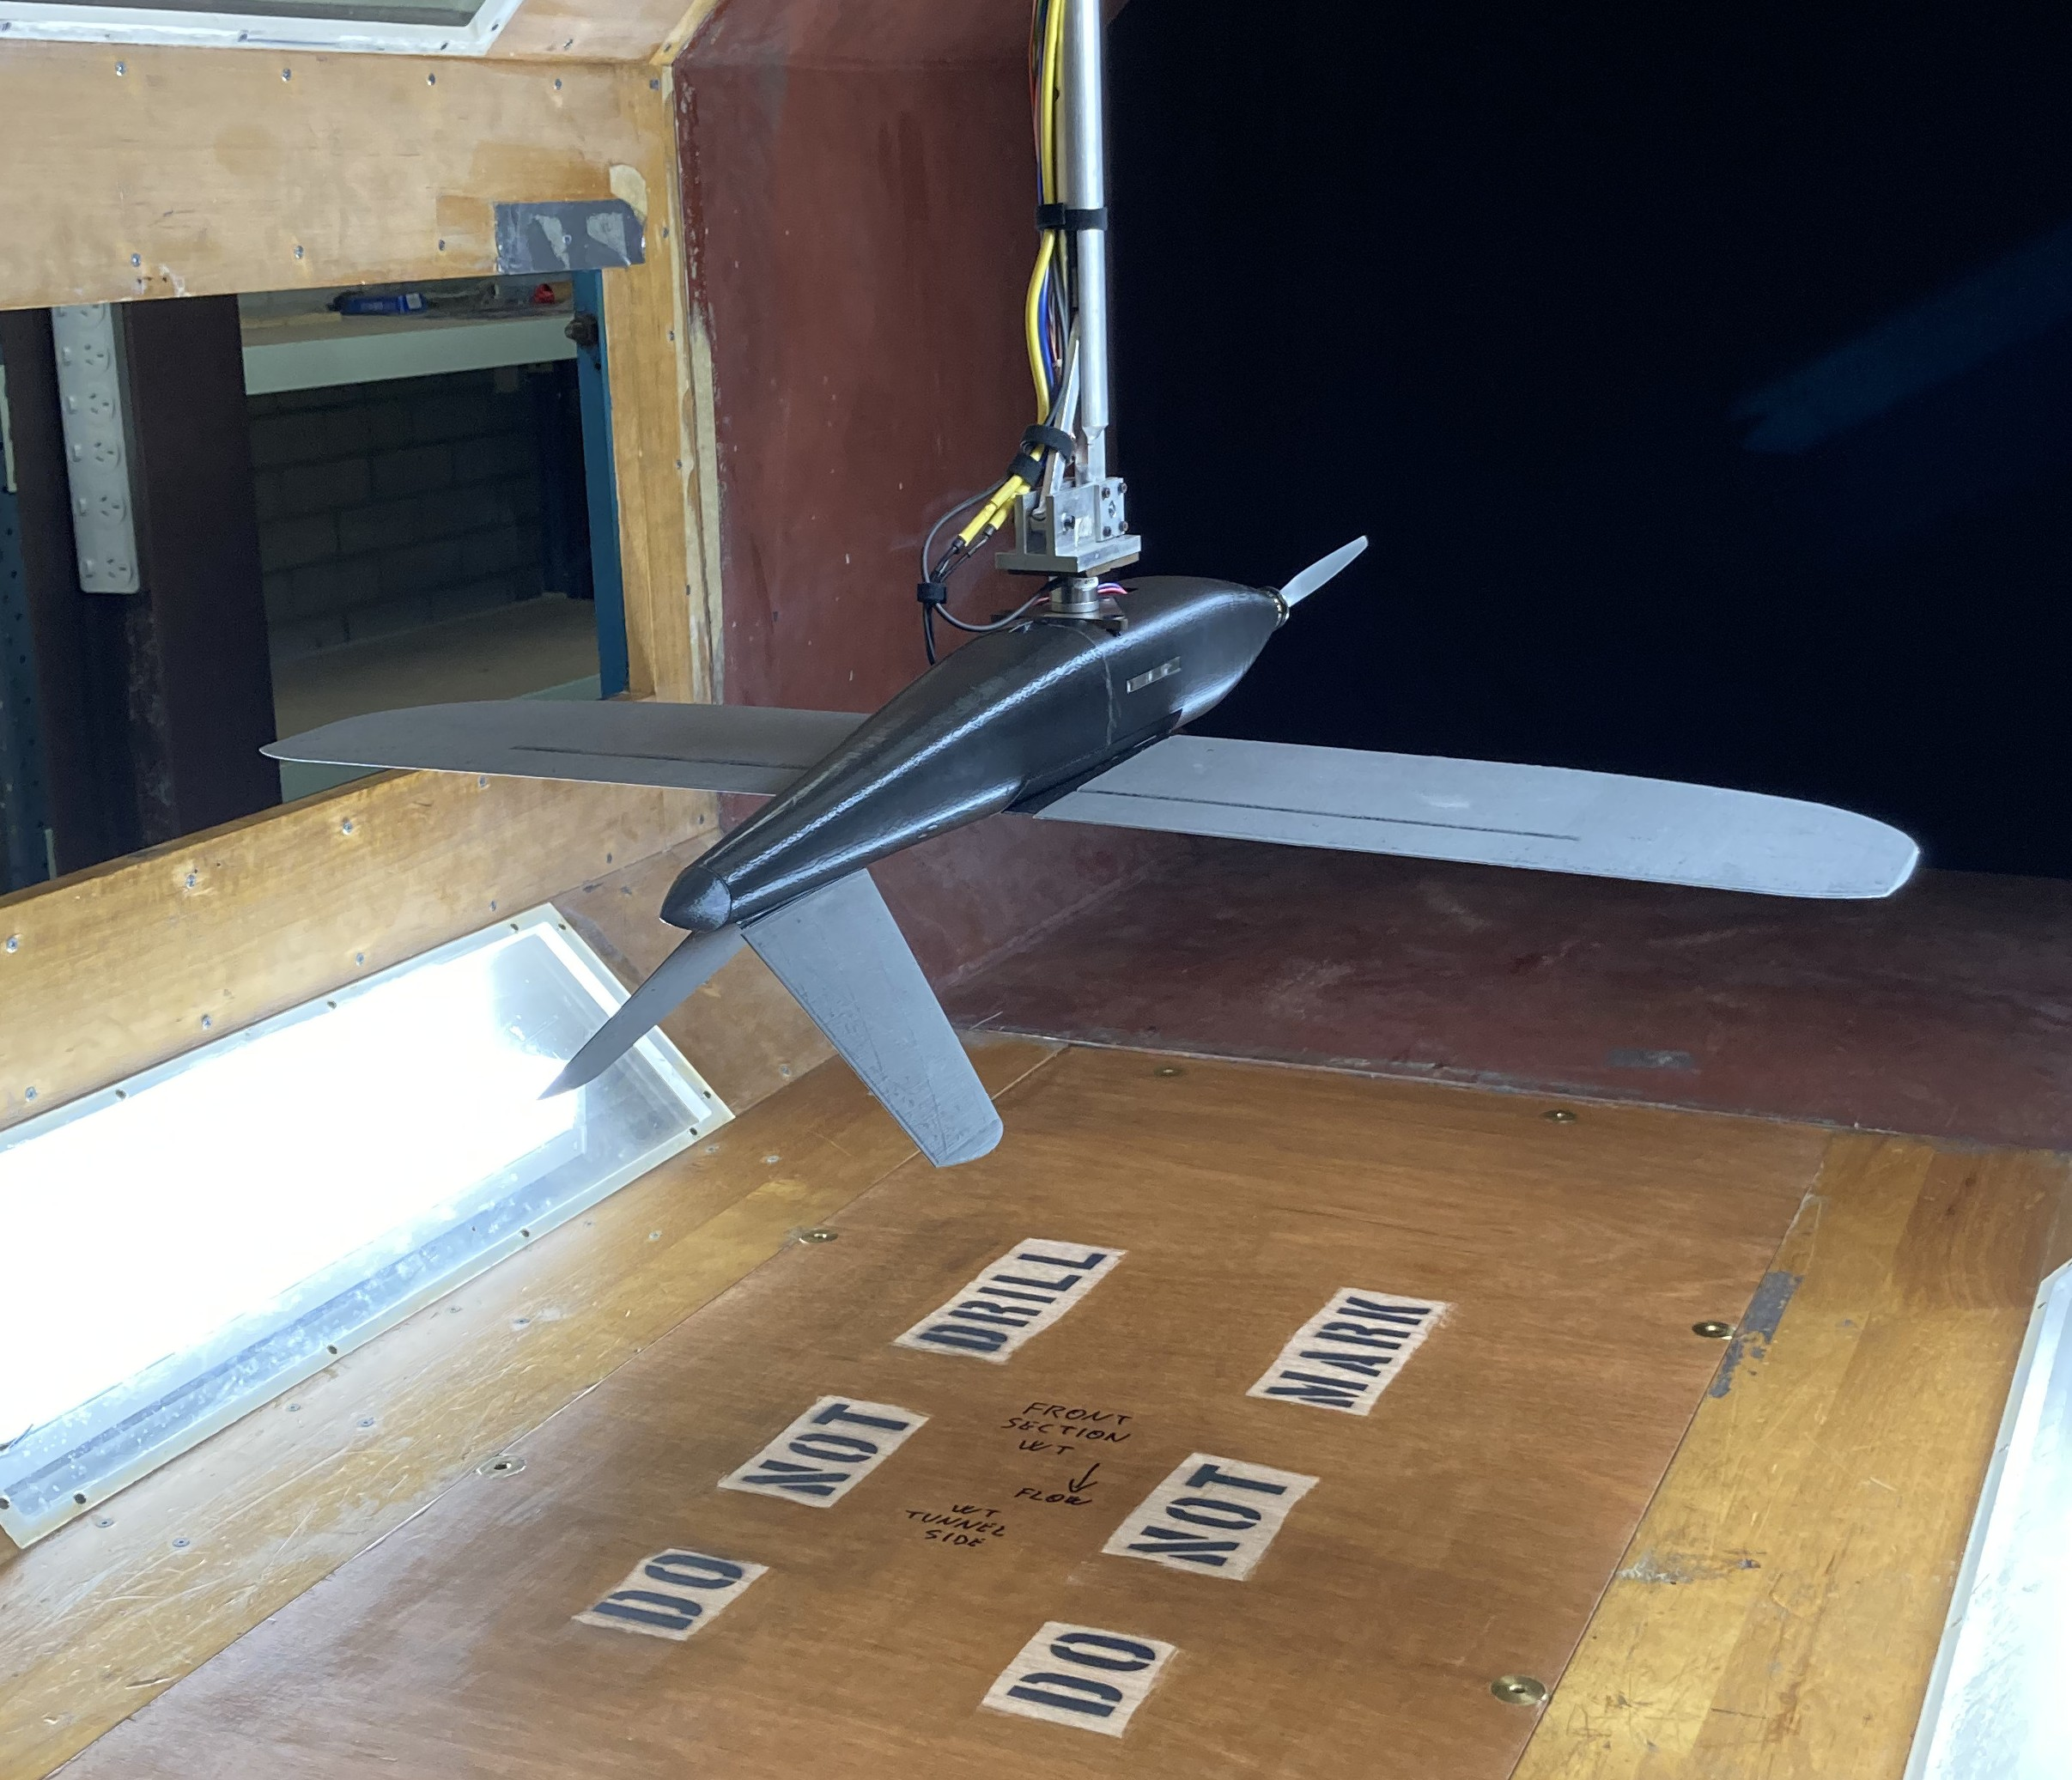
\includegraphics[scale=0.1]{04_Methodology/Figs/tractors}
             \label{fig:tractors}
     \end{subfigure}
        \caption{Examples of MAVs with category}
        \label{fig:typesUsed}
\end{figure}

The wind tunnel was then callibrated for wind speed, atmospheric conditions and angles of attack. The mount used for the model was double checked using a pitch gauge to ensure the angle of attack was correct. 
\begin{figure}
    \centering
    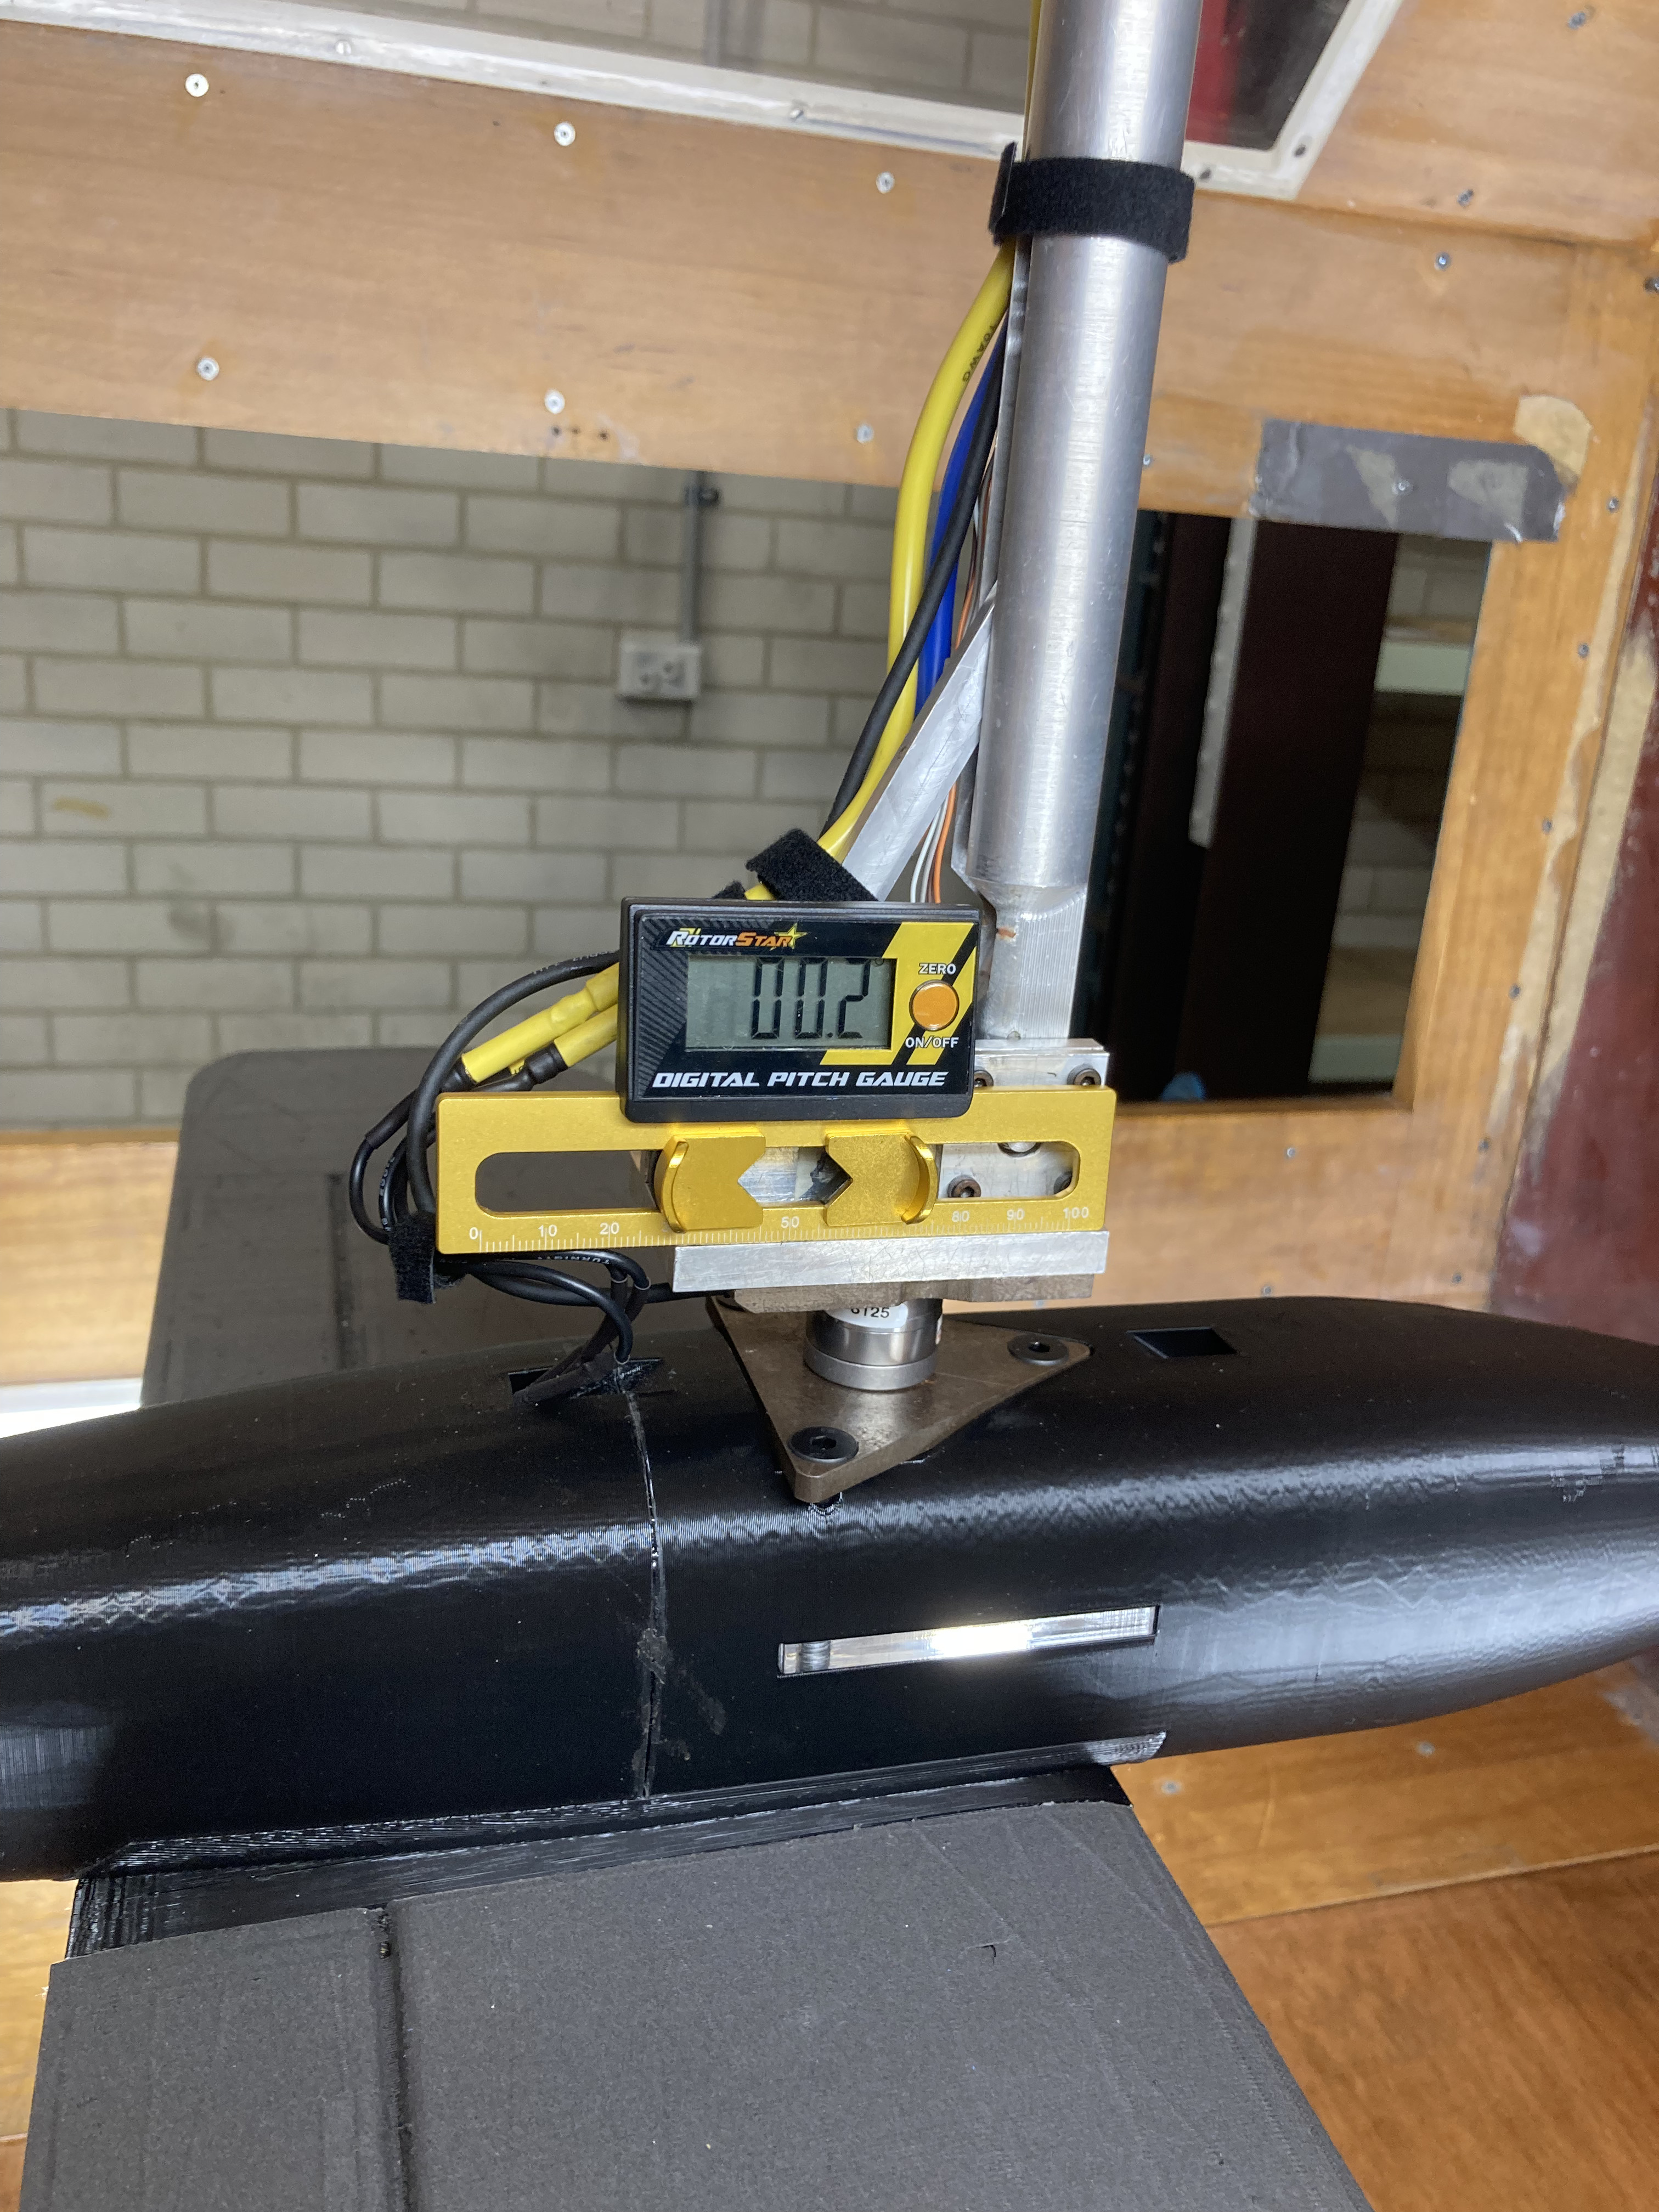
\includegraphics[scale=0.1]{04_Methodology/Figs/pitchGauge.jpg}
    \caption{Callibrating pitch of model mount to ensure Aoa is accurate}
    \label{fig:pitchGauge}
\end{figure}

When using the prop the motor was supplied with a 7.4V battery and the RPM was set to $\approx 6000 RPM$, $\approx 9000RPM$ and $\approx 11000 RPM$. 






\section{Stability Calculation}
In order to determine the stability of the model in all the tested configurations the stability deratives of the model had to be determined. Data from the nano 25 load cell was used to determine the loads and moments acting on the model about the mounting point. These values were transformed \todo{right word?} to the neutral point of the model at 20$\overline{c}$. The aerodynamic coefficients were determined using equations \ref{eqn:lift} to \ref{eqn:drag} and the moment coefficients about the pitch, yaw and roll axis were calculated using Equations \ref{eqn:pitching} to \ref{eqn:yaw}. 





